\section{Transistor models}\label{sec:models}

\subsection{Targets, inputs and metrics}\label{sec:metrics}
The terminal currents span about ten decades ($10^{-15}$ to $10^{-4}$\,A), $I_d$ and $I_s$ change sign, and part of the data is numerical noise
(\cref{sec:data}). The models therefore never predict $I$ directly:
\begin{itemize}
  \item \textbf{Signed-log target} for currents that change sign: $y=\operatorname{asinh}(I/\Ifl)/\ln 10$ with $\Ifl=10^{-15}$\,A. It behaves like
        $\operatorname{sign}(I)\log_{10}(2|I|/\Ifl)$ for $|I|\gg\Ifl$, is linear and exactly zero at $I=0$, and so handles signs, zeros and ten decades
        in one continuous variable.
  \item \textbf{Log target} $y=\log_{10}|I|$ for currents that never change sign (gate current of ON devices, body currents), trained on the rows
        above the floor; the sign is constant and stored with the model.
  \item \textbf{Inputs}: 15 physics-motivated features---$\log_{10}W$, $1000/T$, $\Vdd$, $V_d$, $V_s$, $V_{ds}$, $V_{gs}$, $V_{gd}$, $V_{bs}$, $V_{bd}$,
        $|V_{th0}|$, \texttt{toxe}, $\log_{10}$\texttt{ndep}, \texttt{u0}, \texttt{xj}---standardised to zero mean and unit variance.
\end{itemize}
\textbf{Metrics.} The relative error $(I_{ML}-I_{SPICE})/|I_{SPICE}|$ is evaluated on \emph{resolved} samples, $|I_{SPICE}|>\Ifl$; below the floor
the reference itself is noise. We report the median and the 95th percentile (P95) of its absolute value and its mean (bias). Currents with fewer
than 5\,\% resolved samples (the gate current of OFF devices, which is \emph{never} resolved) are not scored. $R^2$ is computed on the signed-log
target, because on a linear scale it would be dominated by the largest ON currents.

\subsection{Model comparison}\label{sec:comparison}
Four model types were trained and compared for every case (\texttt{scripts/04\_compare\_models.py}). Each predicts the signed log of all four
currents from the 15 features and is trained on the 7{,}000 training rows; every hyper-parameter setting was scored on the validation rows with
score $=\frac12(\text{median}+\text{P95})$ of the relative error, macro-averaged over the scored currents (64 trials in total).
\begin{enumerate}
  \item \textbf{Multi-layer perceptron (MLP)} in PyTorch: 3 hidden layers of 96 or 128 tanh units, float64, Adam (cosine learning-rate decay from
        $3\times10^{-3}$, 1200 epochs, best validation epoch kept), then full-batch L-BFGS polishing.
  \item \textbf{Gradient-boosted trees} (LightGBM): one booster per current, 31 or 127 leaves, learning rate 0.05, early stopping on validation.
  \item \textbf{Kernel ridge regression} with an RBF kernel, $\gamma\in\{0.01,0.03,0.1\}$, $\alpha\in\{10^{-5},10^{-3}\}$.
  \item \textbf{Polynomial ridge regression}, degree 3 or 4, $\alpha\in\{10^{-3},10^{-1},10\}$.
\end{enumerate}
\begin{table}[H]
\centering
{\small
\begin{adjustbox}{max width=\linewidth}
\begin{tabular}{llrrrrl}
\toprule
case & model type & R2 & median err & P95 err & score & best hyper-parameters \\
\midrule
NMOS ON & MLP & 0.9963 & 4.30\% & 22.29\% & 0.1329 & 3 hidden layers x 128 tanh units \\
NMOS ON & LightGBM & 0.9976 & 12.63\% & 61.72\% & 0.3718 & leaves: 31 \\
NMOS ON & Kernel ridge & 0.9281 & 69.44\% & 5359.93\% & 27.15 & gamma: 0.01, alpha: 0.001 \\
NMOS ON & Polynomial ridge & 0.9068 & 71.43\% & 30690.41\% & 153.8 & degree: 4, alpha: 10.0 \\
NMOS OFF & MLP & 0.9951 & 1.69\% & 14.82\% & 0.08256 & 3 hidden layers x 96 tanh units \\
NMOS OFF & LightGBM & 0.9794 & 8.78\% & 63.18\% & 0.3598 & leaves: 31 \\
NMOS OFF & Kernel ridge & 0.9316 & 42.69\% & 161.28\% & 1.02 & gamma: 0.01, alpha: 0.001 \\
NMOS OFF & Polynomial ridge & 0.9302 & 41.67\% & 232.97\% & 1.373 & degree: 4, alpha: 0.1 \\
PMOS ON & MLP & 0.9995 & 2.04\% & 12.16\% & 0.07098 & 3 hidden layers x 96 tanh units \\
PMOS ON & LightGBM & 0.9968 & 13.15\% & 65.96\% & 0.3955 & leaves: 31 \\
PMOS ON & Kernel ridge & 0.9327 & 68.42\% & 4639.72\% & 23.54 & gamma: 0.01, alpha: 0.001 \\
PMOS ON & Polynomial ridge & 0.9137 & 70.11\% & 27706.76\% & 138.9 & degree: 4, alpha: 10.0 \\
PMOS OFF & MLP & 0.995 & 4.29\% & 24.75\% & 0.1452 & 3 hidden layers x 128 tanh units \\
PMOS OFF & LightGBM & 0.9785 & 8.56\% & 65.10\% & 0.3683 & leaves: 31 \\
PMOS OFF & Kernel ridge & 0.9383 & 35.69\% & 151.66\% & 0.9368 & gamma: 0.03, alpha: 0.001 \\
PMOS OFF & Polynomial ridge & 0.9287 & 40.06\% & 187.49\% & 1.138 & degree: 4, alpha: 0.001 \\
\bottomrule
\end{tabular}
\end{adjustbox}
}
\caption{Model comparison on the \emph{validation} set: 4 model types $\times$ 4 cases (best hyper-parameters of each type). $R^2$ on the signed-log target; relative errors on resolved currents ($|I|>10^{-15}$\,A), averaged over the scored currents; score $=\frac12$(median + P95), lower is better. Sorted by score within each case.}
\label{tab:comparison}
\end{table}



\textbf{The MLP is the best model type in all four cases}, with a score 2.5--5 times lower than the runner-up (LightGBM). Kernel ridge and polynomial
ridge assume a smooth global dependence and cannot follow exponential, threshold-like currents over ten decades; their P95 errors reach hundreds to
tens of thousands of percent. Gradient boosting is robust but piecewise constant and cannot reach the precision of the MLP. $R^2$ alone is misleading
here: LightGBM has the higher $R^2$ for NMOS ON, yet a three times larger median error. The MLP was therefore selected for all four cases.

\subsection{From the comparison winner to the final models}\label{sec:final_models}
With the comparison winner (one 4-output MLP per case, trained on 7{,}000 rows) the gate-level mean accuracy was 92.8\,\% (\cref{tab:stages}),
below the target. An analysis of \emph{which} transistor currents determine gate leakage, carried out on transistor data and on the structure of
the gate-level composition (\cref{sec:gates_method}), identified three causes:
\begin{enumerate}
  \item \textbf{Only some currents matter.} The gate leakage is composed from the gate current of ON devices, the channel currents of OFF devices and
        the body currents; the channel current of ON devices is fixed by Kirchhoff's law and never taken from the model (\cref{sec:gates_method}).
        For this low-power card about 98\,\% of the gate leakage at nominal temperature is gate-oxide tunnelling of the ON devices, about 2\,\%
        sub-threshold conduction and about 0.1\,\% junction current. A shared 4-output network spends most of its capacity on ON $I_d/I_s$, which
        the composition does not use.
  \item \textbf{Gates operate at the corners of the input space.} In a gate every drain and source sits at a rail, i.e.\ at a corner of the uniformly
        sampled $(V_d,V_s)$ square, where the training data is sparse and the error of the 4-output model was 2--3 times its average.
  \item \textbf{Effective width.} BSIM4 scales channel and tunnelling currents with $\Weff=W-2\,w_{\mathrm{int}}$ ($w_{\mathrm{int}}=5\,\mathrm{nm}$ in
        both cards), which is only 55\,\% of $W$ at $W=\Lmin$---the width used by the gates.
\end{enumerate}
The final models keep the winning model type (tanh MLP, Adam + L-BFGS) and change how it is used (\texttt{src/dvdml/ml\_v2.py},
\texttt{scripts/05d\_train\_per\_current.py}):
\begin{itemize}
  \item \textbf{one network ensemble per terminal current} ($4$ cases $\times$ $4$ currents $=16$ networks in four model files);
  \item \textbf{width-normalised targets}, $I/(\Weff/\Lmin)$ for $I_d$, $I_g$, $I_s$ and $I/(W/\Lmin)$ for $I_b$ (junction area $\propto W$);
  \item \textbf{six additional physics features}: oxide fields $V_{gs}/t_{ox}$, $V_{gd}/t_{ox}$, $\Vdd/t_{ox}$, gate overdrives $|V_{gs}|-|V_{th0}|$,
        $|V_{gd}|-|V_{th0}|$, and $|V_{th0}|/kT$ (21 inputs in total);
  \item \textbf{training data}: the 7{,}000 training rows plus the 25{,}000 extra uniform rows, and for the currents that dominate leakage
        (ON $I_g$, OFF $I_d/I_s$) the 16{,}000 rail-corner rows (\cref{sec:data});
  \item a fixed sample weight $1+4\,(e(V_d)+e(V_s))$, $e(v)=\exp(-\text{distance to the nearer rail}/0.05\Vdd)$, that emphasises the rails;
  \item \textbf{network}: 4 hidden layers of 128 tanh units (about 52{,}000 weights), Adam in float32 (1500 epochs, batch 512, learning rate
        $3\times10^{-3}$ with cosine decay, best validation state kept), then up to six float64 L-BFGS rounds, each kept only if the validation loss improves;
  \item an \textbf{ensemble} of three networks with different seeds for the leakage-relevant currents (prediction = mean in target space).
\end{itemize}
The settings of the 16 networks are listed in \cref{tab:settings}. Every choice was made on transistor data (validation rows, the uniform hold-out and the
rail-corner hold-out); no gate or circuit SPICE value was used for training, calibration or model selection. \Cref{tab:stages} shows the effect of
the successive changes on the gate and circuit accuracy.
\begin{table}[H]
\centering
{\small
\begin{adjustbox}{max width=\linewidth}
\begin{tabular}{llrrrr}
\toprule
model stage & level & mean accuracy & median err & P95 err & max err \\
\midrule
one 4-output MLP per case, 7k rows & gate (3,600 runs) & 92.79\% & 5.53\% & 19.56\% & 59.36\% \\
one 4-output MLP per case, 7k rows & circuit (51,200 runs) & 92.49\% & 6.38\% & 19.12\% & 46.22\% \\
one MLP per current, I/(W/Lmin) target & gate (3,600 runs) & 96.57\% & 2.39\% & 9.10\% & 38.68\% \\
one MLP per current, I/(W/Lmin) target & circuit (51,200 runs) & 97.90\% & 1.85\% & 3.90\% & 22.78\% \\
+ effective-width target I/(W\_eff/Lmin) & gate (3,600 runs) & 97.63\% & 1.64\% & 5.86\% & 41.46\% \\
+ effective-width target I/(W\_eff/Lmin) & circuit (51,200 runs) & 97.78\% & 1.86\% & 4.85\% & 26.23\% \\
+ rail-corner training rows (final) & gate (3,600 runs) & 99.65\% & 0.19\% & 1.20\% & 5.68\% \\
+ rail-corner training rows (final) & circuit (51,200 runs) & 99.73\% & 0.19\% & 0.79\% & 1.63\% \\
\bottomrule
\end{tabular}
\end{adjustbox}
}
\caption{Gate- and circuit-level accuracy of the successive model stages (same SPICE references, same composition code).}
\label{tab:stages}
\end{table}


\begin{table}[H]
\centering
{\small
\begin{adjustbox}{max width=\linewidth}
\begin{tabular}{lllrll}
\toprule
case & current & target & members & rail-corner data & width normalisation \\
\midrule
NMOS ON & id & asinh (signed log) & 3 & yes & Weff \\
NMOS ON & ig & log10|I| & 3 & yes & Weff \\
NMOS ON & is & asinh (signed log) & 1 & no & Weff \\
NMOS ON & ib & log10|I| & 3 & no & W \\
NMOS OFF & id & asinh (signed log) & 3 & yes & Weff \\
NMOS OFF & ig & asinh (signed log) & 1 & no & W \\
NMOS OFF & is & asinh (signed log) & 3 & yes & Weff \\
NMOS OFF & ib & log10|I| & 3 & no & W \\
PMOS ON & id & asinh (signed log) & 1 & no & Weff \\
PMOS ON & ig & log10|I| & 3 & yes & Weff \\
PMOS ON & is & asinh (signed log) & 1 & no & Weff \\
PMOS ON & ib & log10|I| & 3 & no & W \\
PMOS OFF & id & asinh (signed log) & 3 & yes & Weff \\
PMOS OFF & ig & asinh (signed log) & 1 & no & W \\
PMOS OFF & is & asinh (signed log) & 3 & yes & Weff \\
PMOS OFF & ib & log10|I| & 3 & no & W \\
\bottomrule
\end{tabular}
\end{adjustbox}
}
\caption{Settings of the 16 per-current networks of the final models (all: 21 inputs, 4 hidden layers of 128 tanh units, Adam 1500 epochs + L-BFGS polish).}
\label{tab:settings}
\end{table}



\subsection{Final models on the test set}\label{sec:test}
\Cref{tab:chosen_macro,tab:chosen} report the final models on the 1{,}500 test rows of each case, evaluated once; \cref{fig:pvs} shows predicted
against SPICE currents. The four model files are \texttt{models/<case>.joblib}; their prediction is pure NumPy.
\begin{table}[H]
\centering
{\small
\begin{adjustbox}{max width=\linewidth}
\begin{tabular}{llrrr}
\toprule
case & currents scored & R2 & median err & P95 err \\
\midrule
NMOS ON & id,ig,is,ib & 0.9977 & 6.13\% & 25.41\% \\
NMOS OFF & id,is,ib & 0.9887 & 1.10\% & 6.63\% \\
PMOS ON & id,ig,is,ib & 0.9989 & 2.72\% & 11.31\% \\
PMOS OFF & id,is,ib & 0.9754 & 1.93\% & 10.42\% \\
\bottomrule
\end{tabular}
\end{adjustbox}
}
\caption{Final models on the \emph{test} set (1{,}500 rows per case, evaluated once): macro-average over the scored currents.}
\label{tab:chosen_macro}
\end{table}


\begin{table}[H]
\centering
{\small
\begin{adjustbox}{max width=\linewidth}
\begin{tabular}{llrrrrr}
\toprule
case & current & resolved & R2 & median err & P95 err & bias \\
\midrule
NMOS ON & id & 98.87\% & 0.9981 & 12.69\% & 99.77\% & 21.93\% \\
NMOS ON & ig & 82.20\% & 0.9952 & 0.59\% & 7.22\% & 0.04\% \\
NMOS ON & is & 98.87\% & 0.9978 & 14.69\% & 46.26\% & 7.08\% \\
NMOS ON & ib & 75.93\% & 0.9986 & 0.27\% & 1.63\% & 0.05\% \\
NMOS OFF & id & 53.33\% & 0.9992 & 1.88\% & 9.43\% & -0.02\% \\
NMOS OFF & ig & 0.00\% & -- & -- & -- & -- \\
NMOS OFF & is & 53.80\% & 0.9942 & 1.28\% & 9.59\% & -0.20\% \\
NMOS OFF & ib & 43.47\% & 0.9729 & 0.15\% & 0.86\% & -0.40\% \\
PMOS ON & id & 98.87\% & 0.9987 & 3.91\% & 14.07\% & -0.19\% \\
PMOS ON & ig & 85.20\% & 0.9992 & 0.16\% & 0.75\% & 0.02\% \\
PMOS ON & is & 98.87\% & 0.9994 & 6.47\% & 27.88\% & -1.69\% \\
PMOS ON & ib & 75.13\% & 0.9983 & 0.33\% & 2.55\% & -0.01\% \\
PMOS OFF & id & 54.13\% & 0.9969 & 2.64\% & 15.23\% & -1.38\% \\
PMOS OFF & ig & 0.00\% & -- & -- & -- & -- \\
PMOS OFF & is & 54.60\% & 0.9929 & 2.94\% & 13.80\% & 0.67\% \\
PMOS OFF & ib & 44.33\% & 0.9364 & 0.19\% & 2.23\% & -0.11\% \\
\bottomrule
\end{tabular}
\end{adjustbox}
}
\caption{Final models on the test set, per terminal current (errors on resolved samples, $|I|>10^{-15}$\,A; OFF-state $I_g$ is below the floor in every row and is not scored).}
\label{tab:chosen}
\end{table}



%RETRAIN-PARAGRAPH%

The currents that determine gate leakage are predicted very accurately. On the test rows the ON-state gate current has a median error of
0.2--0.6\,\% and the OFF-state channel currents 1.3--2.9\,\%. At the gate operating points themselves---rail-corner hold-out rows with $V_d$ and $V_s$
exactly at a rail, never used for training or selection---the ON gate current is within 0.07--0.25\,\% and the OFF channel currents within
1.0--2.3\,\% (median, \cref{tab:rails}). The body currents of the ON devices show large relative errors at the exact rails, because with
$V_{bs}=V_{bd}=0$ their junction currents are only just above the $10^{-15}$\,A floor; they contribute about 0.1\,\% of the gate leakage, so these
errors are irrelevant at gate level.
\begin{table}[H]
\centering
{\small
\begin{adjustbox}{max width=\linewidth}
\begin{tabular}{llrrrr}
\toprule
case & current & rows & median err & P95 err & bias \\
\midrule
NMOS ON & ig & 277 & 0.25\% & 1.64\% & -0.23\% \\
PMOS ON & ig & 235 & 0.07\% & 0.26\% & -0.02\% \\
NMOS OFF & id & 194 & 1.35\% & 5.13\% & 0.13\% \\
NMOS OFF & is & 195 & 0.99\% & 3.92\% & -0.20\% \\
PMOS OFF & id & 212 & 1.86\% & 7.51\% & 0.44\% \\
PMOS OFF & is & 212 & 2.29\% & 7.90\% & 0.85\% \\
NMOS ON & ib & 286 & 1.93\% & 49.96\% & -78.48\% \\
PMOS ON & ib & 248 & 1.84\% & 36.36\% & 16.39\% \\
\bottomrule
\end{tabular}
\end{adjustbox}
}
\caption{Error of the final models at the gate operating points: held-out rail-corner rows with $V_d$ and $V_s$ both exactly at $0$ or $V_{DD}$ (never used for training or selection), for the currents that enter the gate leakage.}
\label{tab:rails}
\end{table}



\begin{figure}[!htbp]\centering
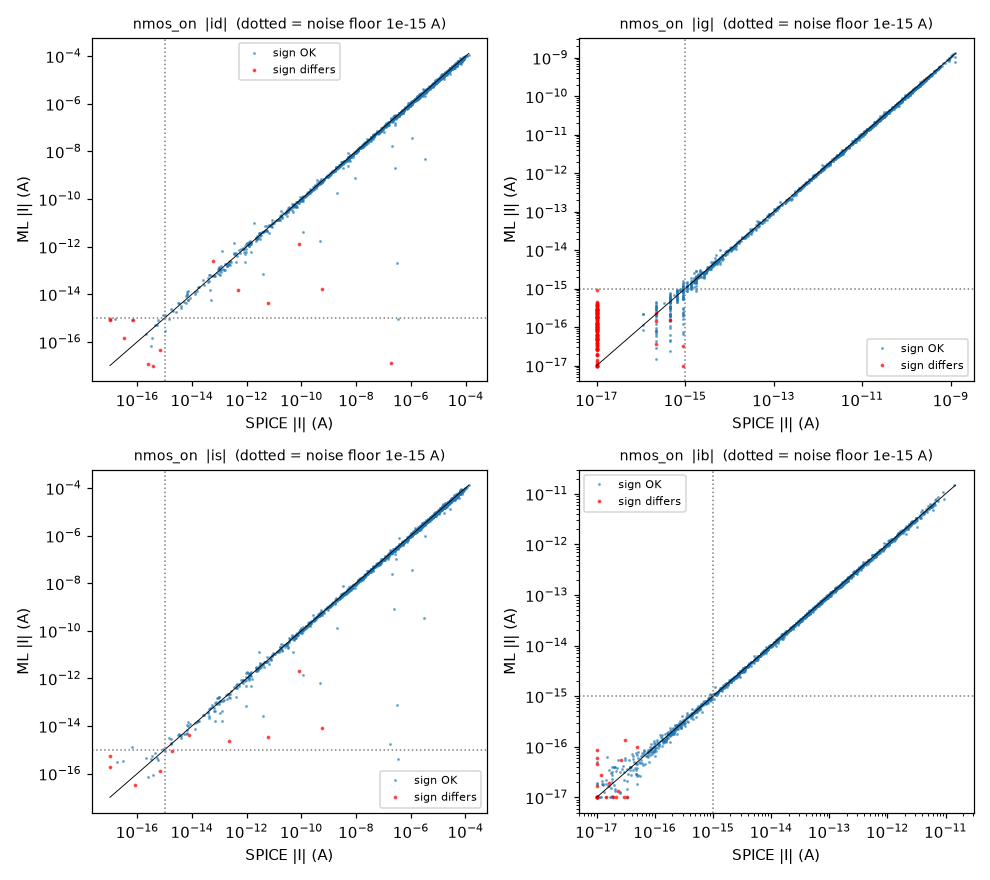
\includegraphics[width=.49\textwidth]{pred_vs_spice_nmos_on.png}\hfill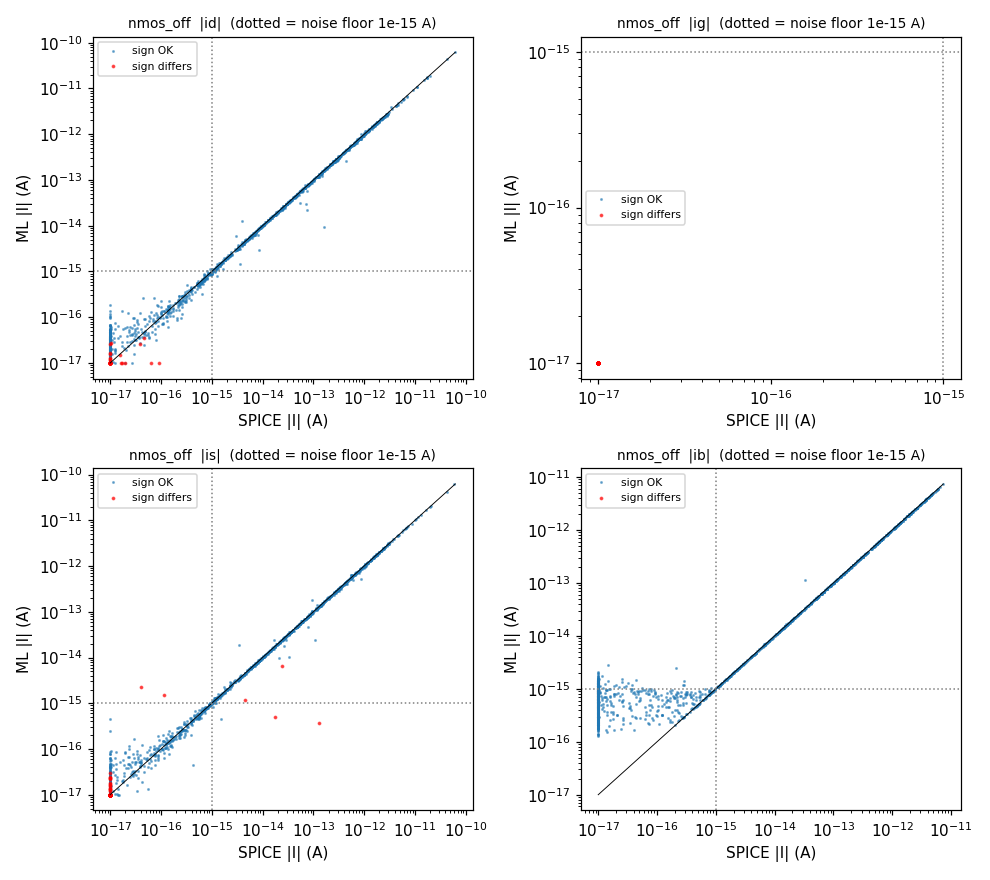
\includegraphics[width=.49\textwidth]{pred_vs_spice_nmos_off.png}\\[0.3em]
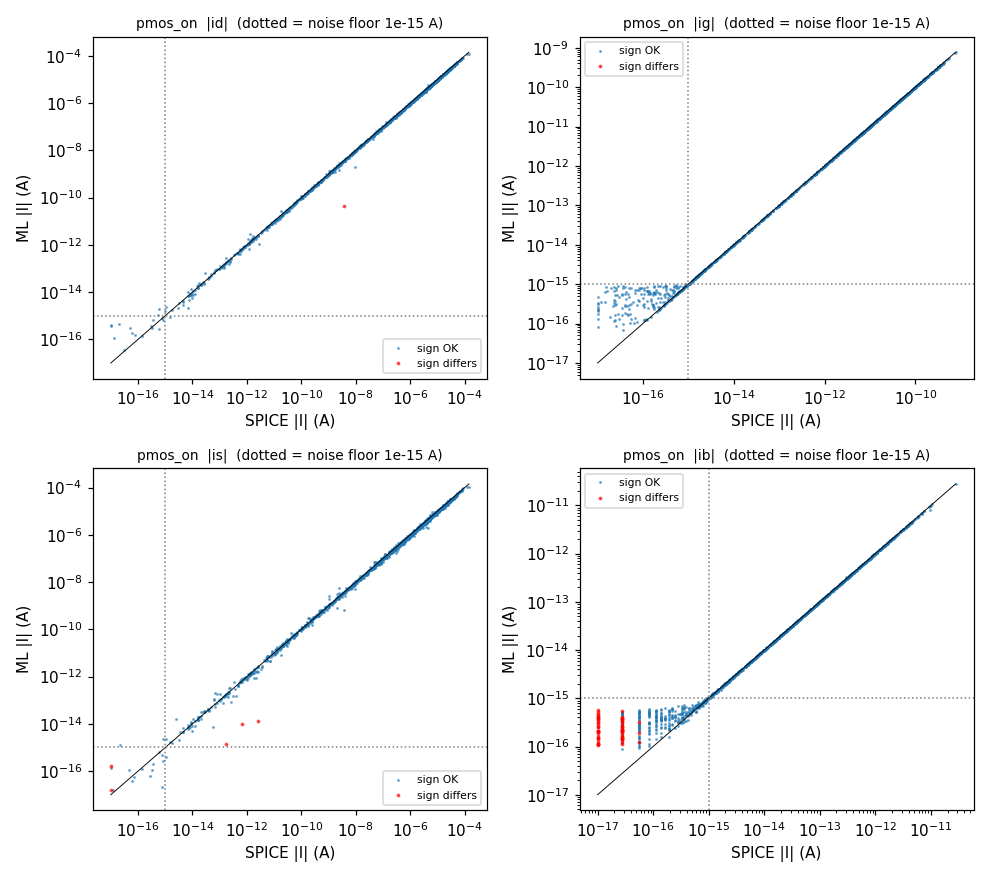
\includegraphics[width=.49\textwidth]{pred_vs_spice_pmos_on.png}\hfill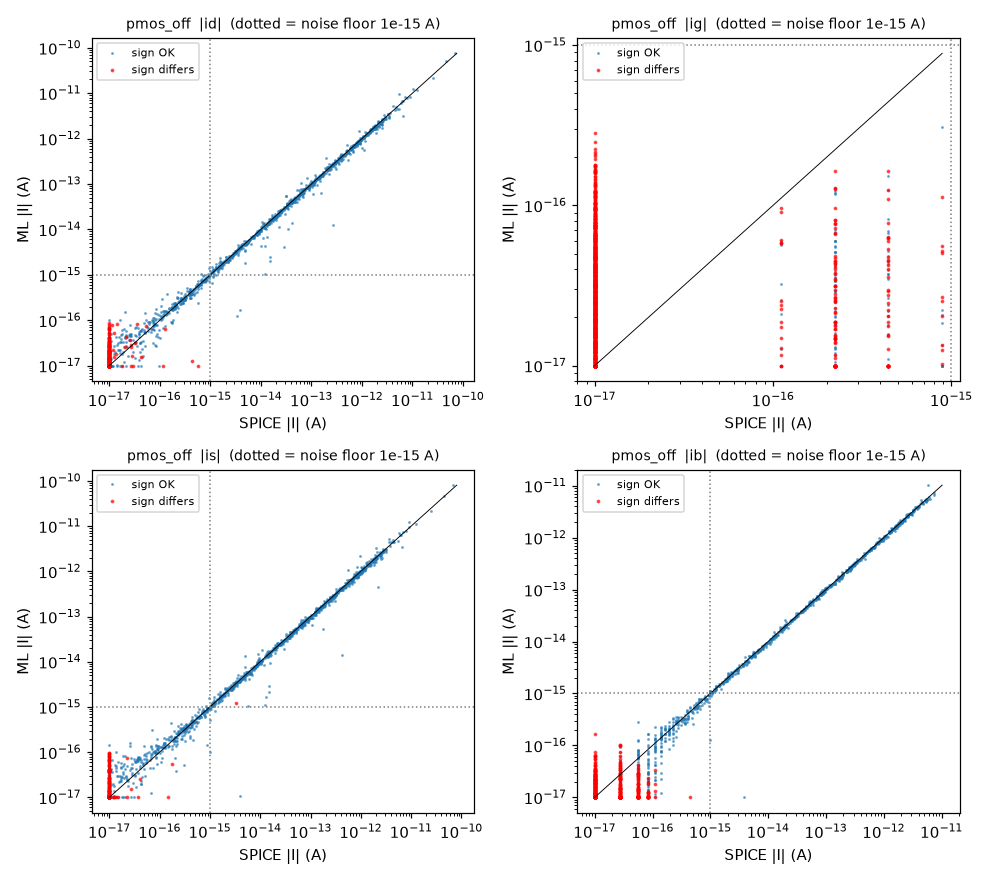
\includegraphics[width=.49\textwidth]{pred_vs_spice_pmos_off.png}
\caption{Predicted versus SPICE terminal currents on the test set for the four final models (absolute values, log axes).}\label{fig:pvs}
\end{figure}

\paragraph{Reason for the final choice.} The MLP was chosen because it was the most accurate model type in all four cases of the validation
comparison (\cref{tab:comparison}). It was then specialised per current, because the gate leakage depends on a few currents at the rail corners of the
input space, and a network devoted to each of these currents---with physically normalised targets and training data where gates operate---is both
more accurate there and still predicts all four terminal currents of every case, as required.
